% Chapter 2

\chapter{Background}\label{chap:background}


\section{Business Field}\label{sec:business}


\section{Fundamentals of Computing for the Studied Area}\label{sec:fundamental}

Equation~\ref{eq:my_equation} is an example of an equation in Latex:

\begin{equation}\label{eq:my_equation}
    h_t = f(W^{(hh)}h_{t-1} + W^{(hx)}x_t).
\end{equation}


Figure\ref{fig:diagram} is an example of including a figure.

\begin{figure}[htb]
    \caption{Simple diagram}
    \centering
    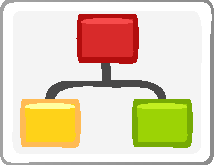
\includegraphics[scale=1.9]{img/diagram.pdf}
    \label{fig:diagram}
    \source{Extracted from \cite{larcc}.}
\end{figure}

\cite{GRIEBLER:IJPP:18}


\cite{MACCOOL:structured_patterns:book:12}


\section{Related Work}\label{sec:rw}


\tablename~\ref{tab:my_table} present an example of a Latex table.

\begin{table}[htb]
    \caption{This is a simple example to build a table.}
    \label{tab:my_table}
    \centering
    \begin{tabular}{|c|c|c|c|}
        \hline
         A & B & N & T\\ 
         \hline
         X & y & W & G\\
         \hline
    \end{tabular}
    
\end{table}